
Extracting the Higgs width from \offshell measurements are performed in ATLAS~\cite{Aaboud:2018puo} and CMS~\cite{CMS:2018bwq} experiments using LHC Run 1 and Run2 data. The latest constraints on the Higgs width are $< 14.4$~MeV and $<9.2$~MeV from ATLAS and CMS, respectively. Theoretical basis of the measurements is that on-shell and off-shell couplings are the same. Developed on the experimental analyses, the expected precision on the Higgs width at the luminosity of 3000~$\fbi$ is given in this section.  

The CMS projection adopted the same analysis strategy as defined in the Run~2 analysis~\cite{CMS-PAS-HIG-18-002}, where the $4\ell$ final state is used. Events are selected and put into different categories that are sensitive to ggF, VBF and VH production modes. The invariant mass of the four leptons, matrix-element based discriminant separating the major signal and background events and discriminants sensitive to the width are used in each category. The ratio between \offshell and \onshell event yields and the shape of the observables are sensitive to the Higgs width. To extrapolate to 3000~$\fbi$, event yields are scaled with luminosity. Assumptions on the uncertainties are made, and two scenarios are considered~\cite{CMS-PAS-FTR-18-011}:
\begin{itemize}
\item {\bf ``Run 2 systematic uncertainties'' scenario (S1):} All systematic uncertainties are kept constant with
  integrated luminosity. The performance of the CMS detector is
  assumed to be unchanged with respect to the reference analysis;

\item {\bf ``YR18 systematic uncertainties'' scenario (S2):} Theoretical uncertainties are scaled down by a factor of two,
  while experimental systematic uncertainties are scaled down with the
  square root of the integrated luminosity until they reach a defined
  minimum value based on estimates of the achievable accuracy with the
  upgraded detector.
\end{itemize} 

The projections are shown in Fig.~\ref{fig:GH-projections}. Limits on \GH are given for an approximate S2 in which the experimental systematics are not reduced, while the theoretical systematics are halved with respect to S1. The $10\%$ additional uncertainty applied on the QCD NNLO K factor on the \glufu background process is kept the same in this approximated S2 in order to remain conservative on the understanding of these corrections on this background component. It is also noted that the uncertainties on the signal and background QCD NNLO K factors are smaller in the Run~2 analysis~\cite{CMS:2018bwq} than in previous projections using Run~1 data~\cite{ATL-PHYS-PUB-2015-024}. The expected \GH precision in S2 is $4.1 ^{+1.0}_{-1.1}$ MeV. 

%%%%%%%%%%%%%%%%%%%%%%%%%%%%%
\begin{figure*}[!htbp]
\centering
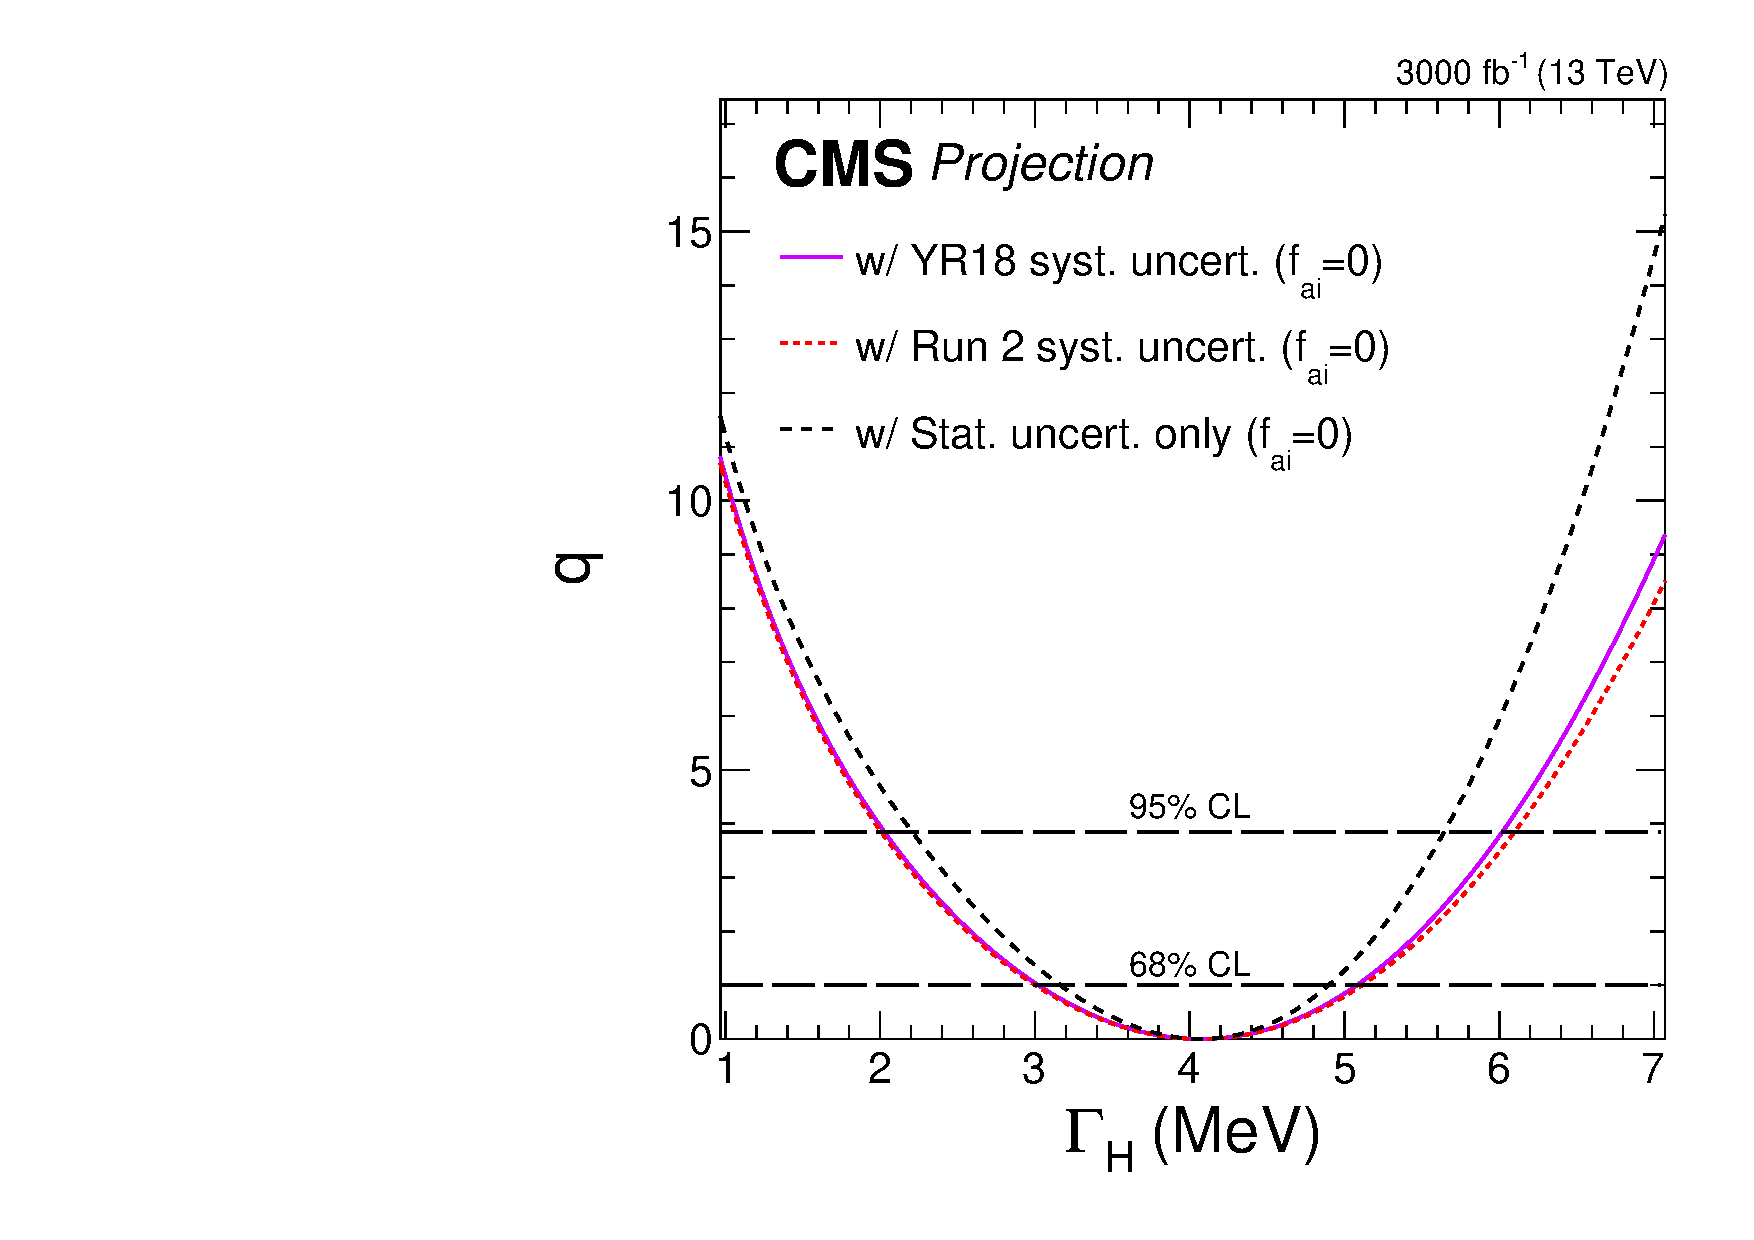
\includegraphics[width=0.45\textwidth]{\main/section5/plots/cCompare_deltaNLLVSGGsm_Proj3000.pdf}
\caption
{
Likelihood scans for projections on \GH at $3000~\fbi$~\cite{CMS-PAS-FTR-18-011}. Scenarios S2 (solid magenta) and S1 (dotted red) are compared to the case where all systematics (dashed black) are removed. The dashed horizontal lines indicate the 68\% and 95\% CLs. 
}
\label{fig:GH-projections}
\end{figure*}
%%%%%%%%%%%%%%%%%%%%%%%%%%%%%


The ATLAS projection~\cite{ATL-PHYS-PUB-2015-024} is based on the ATLAS Run1 analysis~\cite{PhysRevD.91.012006}. $\PH\to\PZ\PZ\to4\ell$ final state is used. Events are selected and put in ggF, VBF and VH categories. The invariant mass of the four leptons and a matrix-element based discriminant sensitive to both signal background separation and width variation are used. In the extrapolation to 3000 $\fbi$, event yields are scaled with luminosity and the change in the center mass of energy. Only theoretical uncertainties are taken into account, as the experimental ones have a negligible impact. The treatment of theoretical uncertainty is close to Run1 analysis, with more conservative ones below: 
\begin{itemize}
	\item {The k-factor uncertainty for the gg initial state signal, background and their interference is taken as 30\%. Based on the latest theory papers, this uncertainty is considered to be conservative, and is 10\% is the CMS projection result.}
	\item {The background to signal k-factor ratio $R^{B}_{H}(\rm{mZZ})$ uncertainty, two benchmarks are considered: 10\% and 30\%. }
\end{itemize}
The expected precision on $\GH$ at 3000 $\fbi$ is $4.2^{+1.5}_{-2.1}$ MeV as shown in Fig.~\ref{ATLAS_projections}. It is more conservative than the CMS result, and the cause of it was discussed above. 
%%%%%%%%%%%%%%%%%%%%%%%%%%%%%
\begin{figure*}[!htbp]
\centering
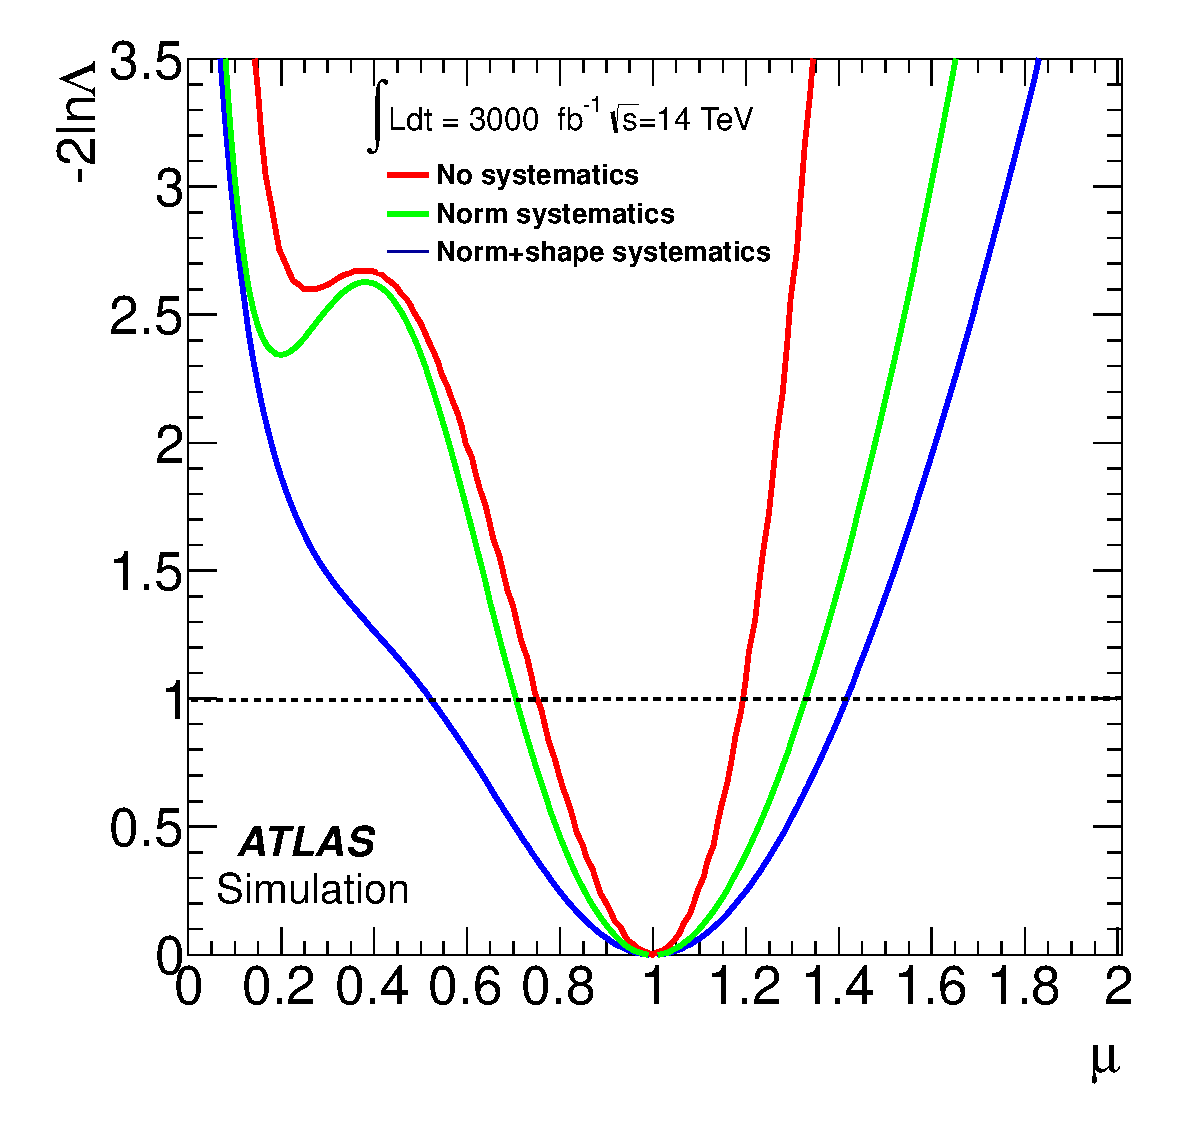
\includegraphics[width=0.45\textwidth]{\main/section5/plots/fig_05b.pdf}
\caption
{
	Likelihood scans on $\mu_{\rm{off-shell}}$ with and without systematic uncertainties. The error on $\mu$ is computed at the $1\sigma$ level and the uncertainty on $R^{B}_{H}(\rm{mZZ})$ is set to 30\%.

}
\label{fig:ATLAS_projections}
\end{figure*}
%%%%%%%%%%%%%%%%%%%%%%%%%%%%%

In conclusion, it is reasonable to believe the realistic precision from ATLAS at 3000~$\fbi$ will be better than the number above. Using the CMS numbers, we con estimate that with CMS and ATLAS measurements combined, the precision on the width can reach $4.1 ^{+0.7}_{-0.8}$ MeV. 

To be added: a conclusion paragraph from theorists